\documentclass[12pt]{article}
\usepackage[english]{babel}
\usepackage{subcaption}
\usepackage{float}
\usepackage{natbib}
\usepackage{url}
\usepackage[utf8x]{inputenc}
\usepackage{amsmath}
\usepackage{graphicx}
\graphicspath{{images/}}
\usepackage{parskip}
\usepackage{fancyhdr}
\usepackage{vmargin}
\usepackage{geometry}
 \geometry{
 a4paper,
 total={170mm,257mm},
 left=20mm,
 top=20mm,
 }

\usepackage{listings}
\usepackage{color} %red, green, blue, yellow, cyan, magenta, black, white
\definecolor{mygreen}{RGB}{28,172,0} % color values Red, Green, Blue
\definecolor{mylilas}{RGB}{170,55,241}


\setmarginsrb{3 cm}{2.5 cm}{3 cm}{2.5 cm}{1 cm}{1.5 cm}{1 cm}{1.5 cm}
\usepackage{listings}
\title{Assignment 1}
\author{Akwasi A. Obeng\newline Eashwar Sathyamurthy \newline Achal P Vyas}                    
\date{December 08, 2019}										
\makeatletter
\let\thetitle\@title
\let\theauthor\@author
\let\thedate\@date
\makeatother

\pagestyle{fancy}
\fancyhf{}
\rhead{\theauthor}
\lhead{\thetitle}
\cfoot{\thepage}

\begin{document}

%%%%%%%%%%%%%%%%%%%%%%%%%%%%%%%%%%%%%%%%%%%%%%%%%%%%%%%%%%%%%%%%%%%%%%%%%%%%%%%%%%%%%%%%%

\lstset{language=Matlab,%
    %basicstyle=\color{red},
    breaklines=true,%
    morekeywords={matlab2tikz},
    keywordstyle=\color{blue},%
    morekeywords=[2]{1}, keywordstyle=[2]{\color{black}},
    identifierstyle=\color{black},%
    stringstyle=\color{mylilas},
    commentstyle=\color{mygreen},%
    showstringspaces=false,%without this there will be a symbol in the places where there is a space
    numbers=left,%
    numberstyle={\tiny \color{black}},% size of the numbers
    numbersep=9pt, % this defines how far the numbers are from the text
    emph=[1]{for,end,break},emphstyle=[1]\color{red}, %some words to emphasise
    %emph=[2]{word1,word2}, emphstyle=[2]{style},    
  }


\begin{titlepage}
	\centering
    \vspace*{0.5 cm}
    
\includegraphics[scale = 0.1]{uon.jpeg}\\[1.0 cm]	% University Logo
    \textsc{\LARGE ENPM673(Robot Perception)}\\[2.0 cm]	% University Name
	\textsc{\Large Formal Report}\\[0.5 cm]				% Course Code
	\textsc{\large Project}\\[0.5 cm]				% Course Name
	\rule{\linewidth}{0.2 mm} \\[0.4 cm]
	{ \huge \bfseries \thetitle}\\
	\rule{\linewidth}{0.2 mm} \\[1.5 cm]
	
	\begin{minipage}{0.4\textwidth}
		\begin{flushleft} \large
			\emph{Author:}\\
			\theauthor
			\end{flushleft}
			\end{minipage}~
			\begin{minipage}{0.4\textwidth}
			\begin{flushright} \large
			\emph{DirectoryID:} \\
			obenga01 \\ eashwar  \\ avyas
		\end{flushright}
	\end{minipage}\\[2 cm]
	
	{\large \thedate}\\[2 cm]
 
	\vfill
	
\end{titlepage}

%%%%%%%%%%%%%%%%%%%%%%%%%%%%%%%%%%%%%%%%%%%%%%%%%%%%%%%%%%%%%%%%%%%%%%%%%%%%%%%%%%%%%%%%%

\tableofcontents
\pagebreak

%%%%%%%%%%%%%%%%%%%%%%%%%%%%%%%%%%%%%%%%%%%%%%%%%%%%%%%%%%%%%%%%%%%%%%%%%%%%%%%%%%%%%%%%%

\section{Problem1- Detection}
We need to encode the given AR tag which is represented in 8x8 grid by detecting the innermost 2x2 grid to get the tag id which should be affected by the camera rotation.
\begin{figure}[h]
    \centering
    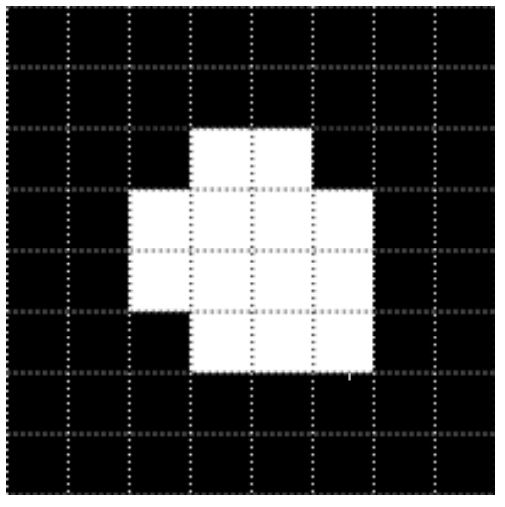
\includegraphics[width=6cm]{artaggrid}
    \caption{Grid view of AR tag}
    \label{fig:artaggrid}
\end{figure}
\subsection{Procedure followed to solve Problem 1:}
\begin{enumerate}
\item First we need the compute homography matrix of the corners of the AR tag to warp the image. Homography is done is using the
\begin{equation}
homography(worldcoordinates, pixelcoordinates)
\end{equation}
function in the python file which uses the inbuild $svd()$ function to get the required vector. The n normalizing the obtained vector and reshaping it to 3x3 matrix to get the homography matrix.
We have verified the coded homography matrix with in-build functions and got the same results.
\begin{figure}[h]
    \centering
    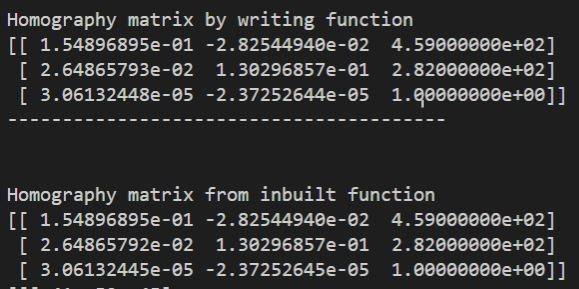
\includegraphics[width=12cm]{homography}
    \caption{Homography matrix verification}
    \label{fig:homography}
\end{figure}

\item After finding the homography matrix, we warped the AR tag image by multiplying every pixel with the homography matrix. We did not get perfect results in this part as there were white spots(holes) in the picture. 

\item After warping, we encoded the tag for our id by performing operations on inner 2x2 grid. Given below are the comparisons of the output images got using running opencv function and our warping function.
\begin{figure}[h]
    \centering
    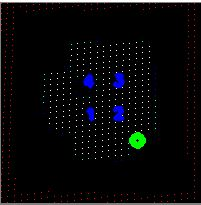
\includegraphics[width=8cm]{warping_coded}
    \caption{Output from developed warping function}
    \label{fig:warping_coded}
\end{figure}
We get white spots(holes) as opposed to a uniform color distribution when using the warping function developed. To improve this,
we look at the neighborhood of neighboring pixels to determine the orientation of the AR tag. However, this is still not robust and as precise as the inbuilt function utilized in opencv, hence the orientation of AR tag shifts sometimes.
\begin{figure}[h]
    \centering
    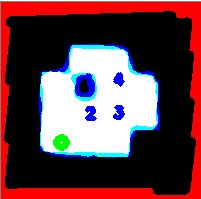
\includegraphics[width=8cm]{warping_opencv}
    \caption{Output from inbuilt opencv function}
    \label{fig:warping_coded}
\end{figure}
\begin{center}
    1 represents the least significant bit\\
    4 represents the most significant bit \\
    Tag id is calculated in clockwise direction starting from 1 to 4
\end{center}
\item The snippets of the video is given below. The snippet shows the tag id in blue color.
\begin{figure}[h]
    \centering
    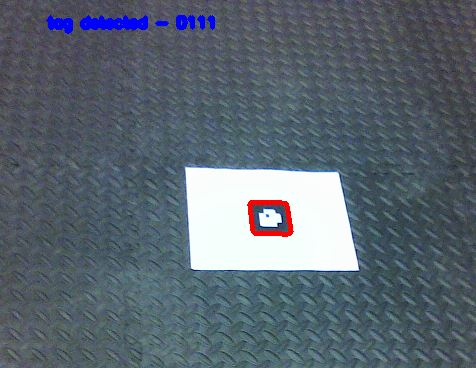
\includegraphics[width=10cm]{tag_id_outputvideo0}
    \caption{Tag id detection for video Tag1}
    \label{fig:Tag id output}
\end{figure}

\begin{figure}[h]
    \centering
    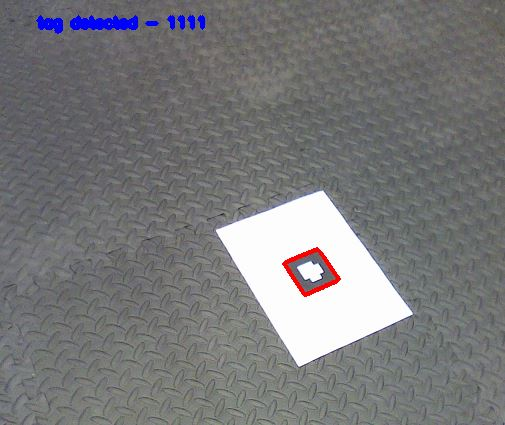
\includegraphics[width=10cm]{tag_id_outputvideo1}
    \caption{Tag id detection for video Tag0}
    \label{fig:Tag id output}
\end{figure}

\end{enumerate}
\subsection{Difficulties Faced:}
\begin{enumerate}
\item The main difficult part was building the custom warping function. Even though we could warp the image, there were many holes present which made the AR tag id decoding difficult.
\end{enumerate}



\section{Problem2 - Tracking}
\subsection{Problem 2a - Superimposing an image onto the tag}
\subsection{Procedure for solving problem }
\begin{enumerate}
\item First from problem 1, we obtained four corners of the AR tag. We used those AR tag corner coordinates and performed homography between corners of the Lena image and AR tag corners.
\item $homography(worldcoordinates, pixelcoodinates)$ in detection.py python file is used to compute the homography. The function takes 2 list as arguments and returns a 3x3 homography matrix.The Lena image corners were obtained $shape()$ function in opencv which gives the $[height, width]$ of the image.


\item After performing homography, we developed a $warping()$ function which warps all the pixels of Lena image onto the ARtag by multiplying each pixel with the homography matrix. First, the image is placed in correct orientation of the tag and then warped.

\item The following are the output snippets of the tag being superimposed on AR tag on different videos.
\begin{figure}[h]
    \centering
    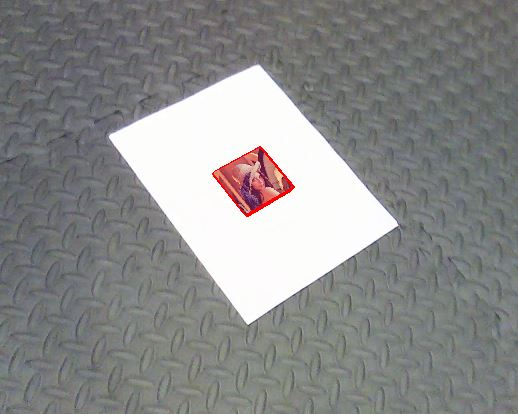
\includegraphics[width=10cm]{Tag0_videooutput}
    \caption{Superimposing Lena onto AR tag on Tag0 video}
    \label{fig:video frame output}
\end{figure}

\begin{figure}[h]
    \centering
    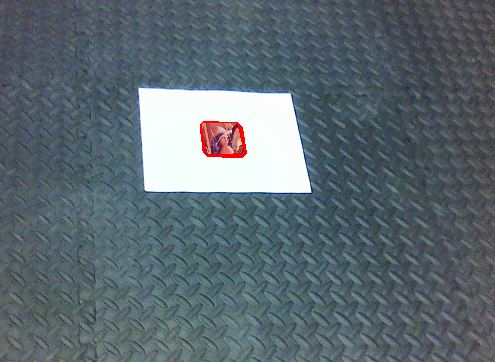
\includegraphics[width=10cm]{Tag1_videooutput}
    \caption{Superimposing Lena onto AR tag on Tag1 video}
    \label{fig:video frame output}
\end{figure}
\newpage
\begin{figure}[h]
    \centering
    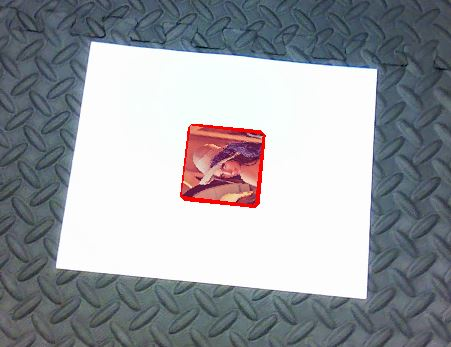
\includegraphics[width=10cm]{Tag2_videooutput}
    \caption{Superimposing Lena onto AR tag on Tag2 video}
    \label{fig:video frame output}
\end{figure}
\end{enumerate}
\subsection{Difficulties Faced:}
\begin{enumerate}
\item We faced a few problem in detecting edges. Sometimes the code detected the edges of the white paper and the image would get superimposed on the entire white paper instead of the ARtag.
\end{enumerate}
\newpage


\subsection{Problem 2(b) - Placing a virtual cube on the tag}
\subsection{Procedure for solving problem }
\begin{enumerate}
\item First we computed the homography between the world coordinates and image plane of the AR tag.

\item Next we coded for obtaining the projection matrix from the homography matrix.

\item Then we wrapped the world coordinates of the AR tag onto the image plane. 

\item Then we found out the projection matrix from the homography matrix.

\item Then we project the 8 3-D cube coordinates of the cube onto the image plane by multiplying with the projection matrix and converting it into the homogenous coordinates by dividing the 3-D point with its z-coordinate.

\item The following are the snippets of output from three videos.
\end{enumerate}
\begin{figure}[h]
    \centering
    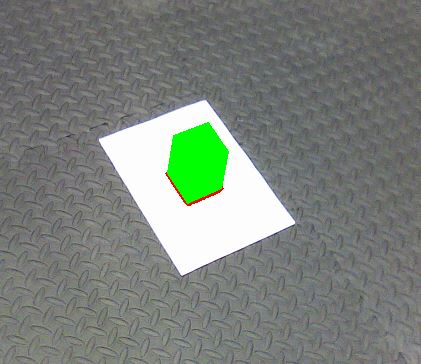
\includegraphics[width=6cm]{Tag0_cube}
    \caption{3D cube superimpose on Tag0 video}
    \label{fig:video frame output}
\end{figure}

\begin{figure}[h]
    \centering
    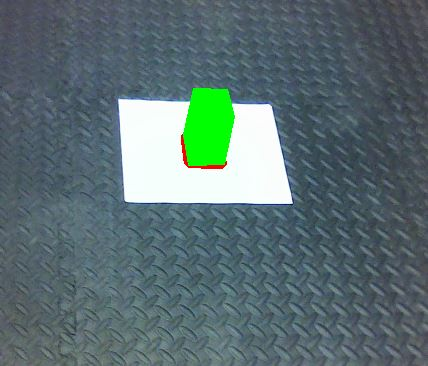
\includegraphics[width=8cm]{Tag1_cube}
    \caption{3D cube superimpose on Tag1 video}
    \label{fig:video frame output}
\end{figure}
\newpage
\begin{figure}[h]
    \centering
    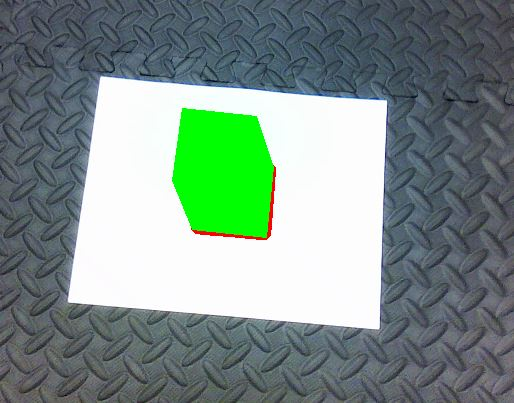
\includegraphics[width=8cm]{Tag2_cube}
    \caption{3D cube superimpose on Tag2 video}
    \label{fig:video frame output}
\end{figure}
\subsection{Difficulties Faced:}
\begin{enumerate}
\item We faced a lot for problem in the projection matrix and converting the 3-D coordinates of the cube to 8 2-D homogenous coordinates.
\end{enumerate}
\end{document}



